%*******10********20********30********40********50********60********70********80
\clearpage
\subsection{Expansion Intensified Part Range Related to Behavior of Concrete During DEF Expansion}




\begin{figure}[!ht]
\centering
    %*******
    \begin{subfigure}{.33\textwidth}
      \centering
      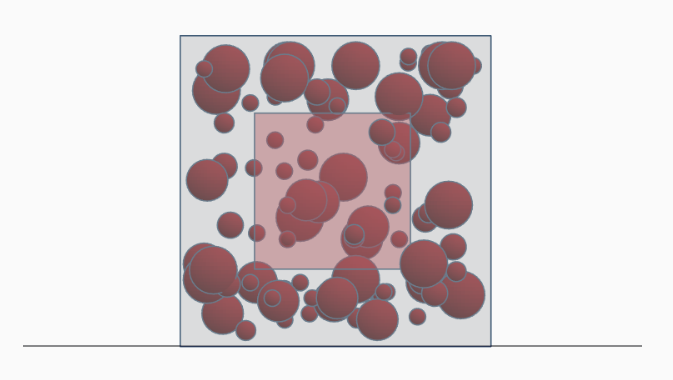
\includegraphics[width=.8\linewidth]{Files/DEF_X/X0_3ds.png}
      \caption{Intensified $50 \times 50 \times 50$ mm Case\\ Cross Section}
    \end{subfigure}%
    %*******
    \begin{subfigure}{.33\textwidth}
      \centering
      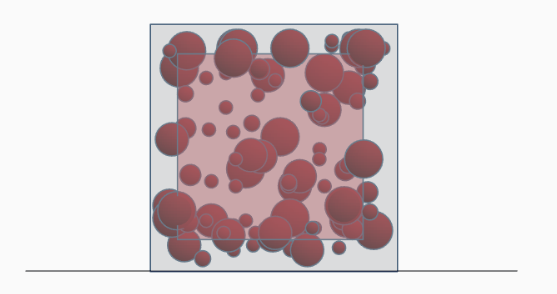
\includegraphics[width=.8\linewidth]{Files/DEF_X/X-5_3ds.png}
      \caption{Intensified $75 \times 75 \times 75$ mm Case \\ Cross Section}
    \end{subfigure}%
    %*******
    \begin{subfigure}{.33\textwidth}
      \centering
      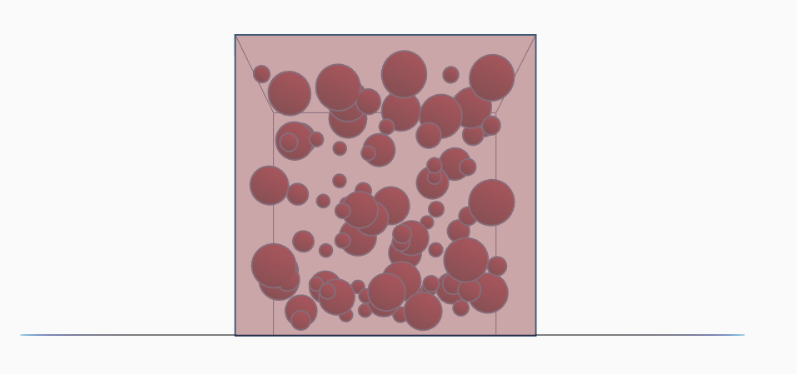
\includegraphics[width=.9\linewidth]{Files/DEF_X/X-1_3ds.png}
      \caption{Intensified $100 \times 100 \times 100$ mm Case\\ Cross Section}
    \end{subfigure}
    %*******
  \caption{DEF intensified part range}
  \label{fig:DEF_Xdddd}
\end{figure}

In this section, DEF expansion simulation result of intensified center $75 \times 75 \times 75$ mm and uniformly expansion for all part (intensified center $100 \times 100 \times 100$ mm) is presented (Figure \ref{fig:DEF_Xdddd}).

\subsubsection{Expansion Intensified $75 \times 75 \times 75$ mm at Center of Model}

In Tabel \ref{table:DEF_Xaa-5_EXP} and Figure \ref{fig:DEFA30X0vzzsX-5_exp} the relationship between initial strain giving and global expansion is presented. With increasing of initial strain, global expansion both increase linearly, but with different speed in smaller and larger expanding intensified range. Since more interfaced are given large expansion in $75 \times 75 \times 75$ mm case, it is reasonable that larger global expansion should be achieved.

From Figure \ref{fig:DEF_A30X-ss1C_3D}, Figure \ref{fig:ASR_A30X-5ssC_3DS}, and Figure \ref{fig:DEF_A30X-5C_3Dasdasd}, it can be seen that when intensified the DEF expansion at the center $75 \times 75 \times 75$ mm, still the characteristic map cracking pattern can be achieved, which is similar to $50 \times 50 \times 50$ mm case.

\begin{table}[ht!]
  \caption{One Dimensional Expansion Ratio[\%] in Expansion Intensified $75 \times 75 \times 75$ mm at Center of Model DEF Model Simulation}
\centering
\begin{tabular}{ ||p{2cm}|p{2cm}|p{2cm}| }
 \hline
    Initial Strain (Each Step) & Expanding Steps &  Final Expansion[\%] \\ [0.5ex]
 \hline\hline
  0 & 0 & 0  \\
  0.001 & 20 & 0.1671 \\
  0.002 & 20 & 0.3380 \\
  0.003 & 20 & 0.5118 \\
  0.005 & 20 & 0.8577 \\
 \hline
\end{tabular}

\label{table:DEF_Xaa-5_EXP}
\end{table}

\begin{figure}[ht!]
\centering
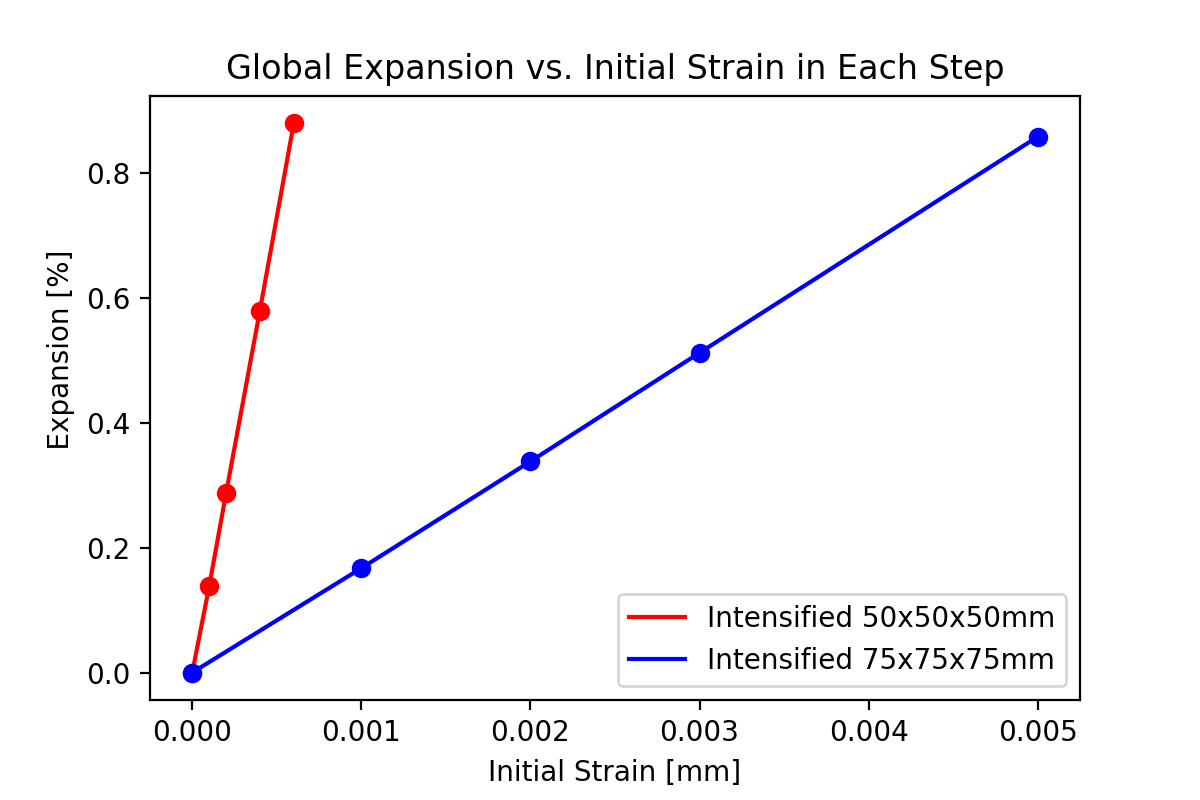
\includegraphics[width=.8\linewidth]{Files/exp_plot/DEFA30X0vsX-5_exp.png}
  \caption{Global Expansion vs. Initial Strain Given in Each Step}
  \label{fig:DEFA30X0vzzsX-5_exp}
\end{figure}

% Surface
\begin{figure}[!h]
\centering

    %*******
    \begin{subfigure}{.5\textwidth}
      \centering
      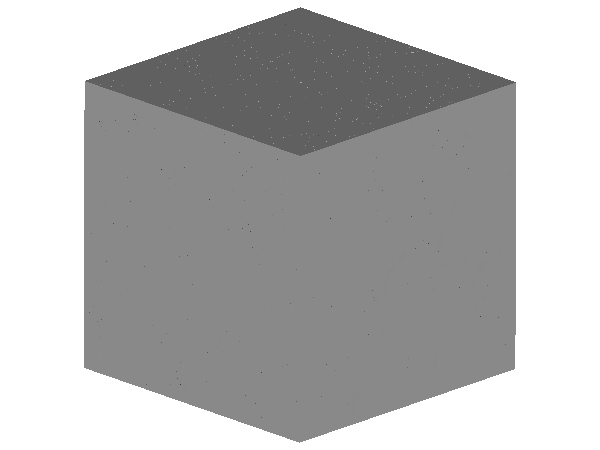
\includegraphics[width=.8\linewidth]{Files/exp_3D/ASR/A30Undamaged.png} %TODO: Fix. Should be A30
    \caption{Case 0: 0\% Expansion}
    \end{subfigure}%
    %*******
    \begin{subfigure}{.5\textwidth}
      \centering
      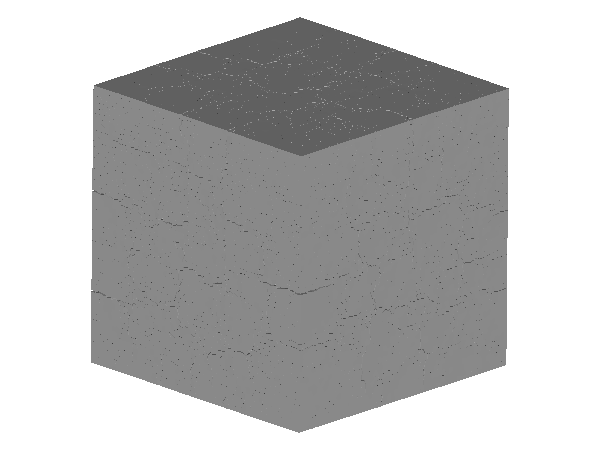
\includegraphics[width=.8\linewidth]{Files/exp_3D/DEF/A30X-5C_1_3d.png}
    \caption{Case 1: 0.1671\% Expansion}
    \end{subfigure}
    %*******
    \begin{subfigure}{.5\textwidth}
      \centering
      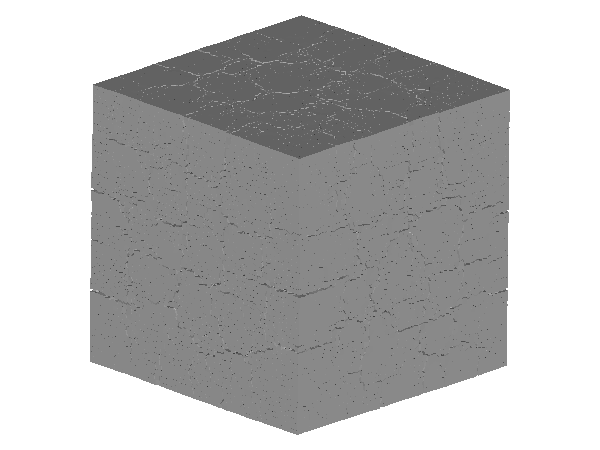
\includegraphics[width=.8\linewidth]{Files/exp_3D/DEF/A30X-5C_2_3d.png}
    \caption{Case 2: 0.3380\% Expansion}
    \end{subfigure}%
    %*******
    \begin{subfigure}{.5\textwidth}
      \centering
      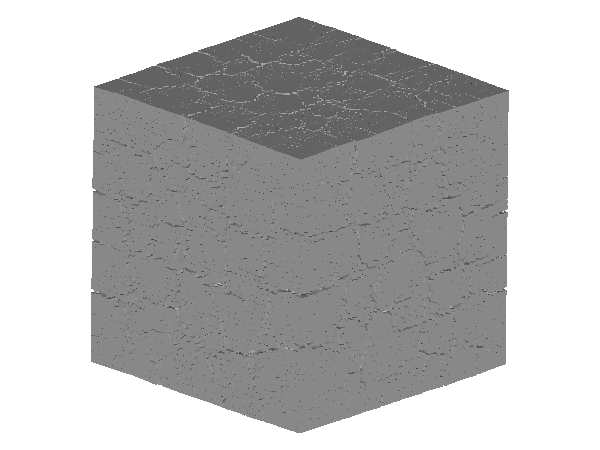
\includegraphics[width=.8\linewidth]{Files/exp_3D/DEF/A30X-5C_3_3d.png}
    \caption{Case 3: 0.5118\% Expansion}
    \end{subfigure}
    %*******
    \begin{subfigure}{.5\textwidth}
      \centering
      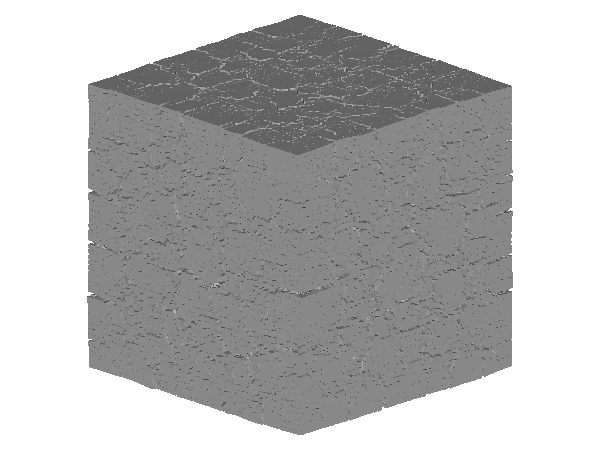
\includegraphics[width=.8\linewidth]{Files/exp_3D/DEF/A30X-5C_4_3d.png}
    \caption{Case 4: 0.8577\% Expansion}
    \end{subfigure}%
    %*******

  \caption{3D Surface Cracks Expansion Intensified $75 \times 75 \times 75$ mm ($Deformation \times 10$)}
  \label{fig:DEF_A30X-ss1C_3D}
\end{figure}

% Surface of one side
\begin{figure}[!h]
\centering

    %*******
    \begin{subfigure}{.5\textwidth}
      \centering
      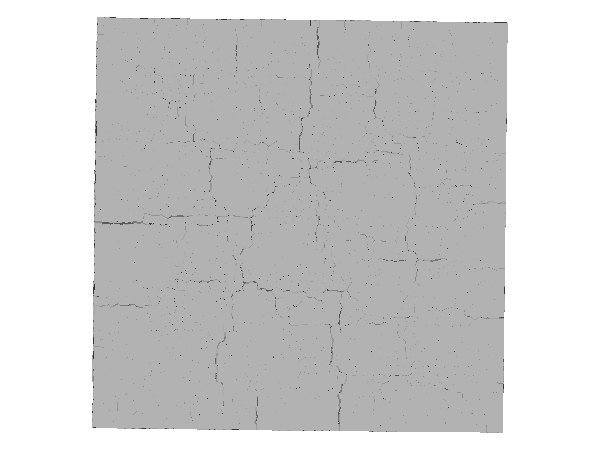
\includegraphics[width=.8\linewidth]{Files/exp_3D/DEF/A30X-5C_1_3ds.png}
    \caption{Case 0: 0\% Expansion}
    \end{subfigure}%
    %*******
    \begin{subfigure}{.5\textwidth}
      \centering
      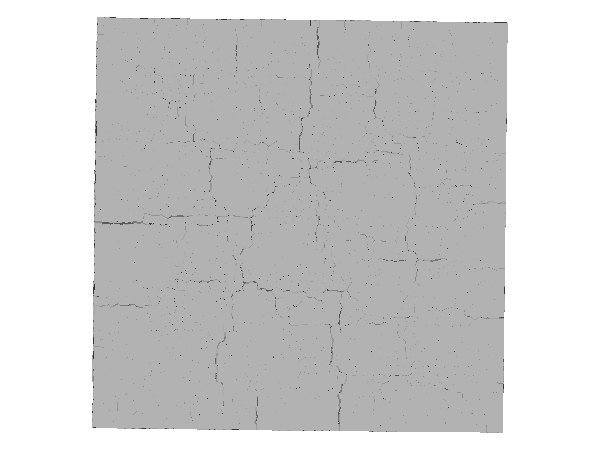
\includegraphics[width=.8\linewidth]{Files/exp_3D/DEF/A30X-5C_1_3ds.png}
    \caption{Case 1: 0.1671\% Expansion}
    \end{subfigure}
    %*******
    \begin{subfigure}{.5\textwidth}
      \centering
      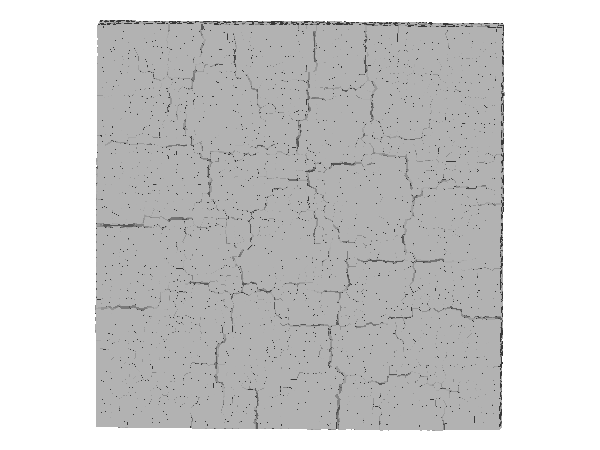
\includegraphics[width=.8\linewidth]{Files/exp_3D/DEF/A30X-5C_2_3ds.png}
    \caption{Case 2: 0.3380\% Expansion}
    \end{subfigure}%
    %*******
    \begin{subfigure}{.5\textwidth}
      \centering
      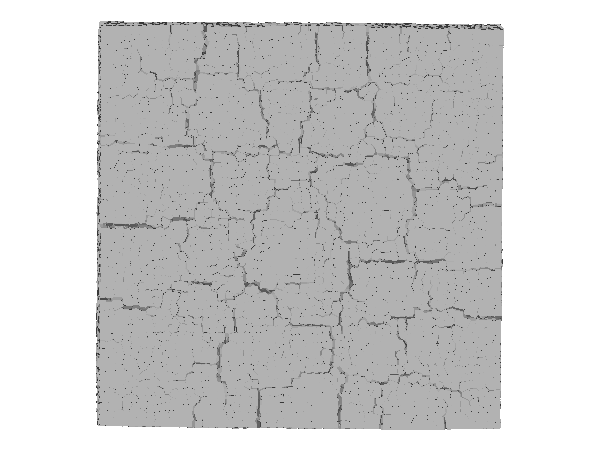
\includegraphics[width=.8\linewidth]{Files/exp_3D/DEF/A30X-5C_3_3ds.png}
    \caption{Case 3: 0.5118\% Expansion}
    \end{subfigure}
    %*******
    \begin{subfigure}{.5\textwidth}
      \centering
      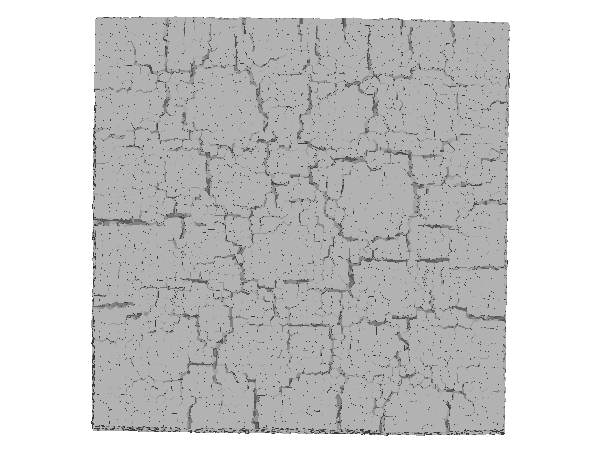
\includegraphics[width=.8\linewidth]{Files/exp_3D/DEF/A30X-5C_4_3ds.png}
    \caption{Case 4: 0.8577\% Expansion}
    \end{subfigure}%

  \caption{3D Surface Cracks (Single Side View) Expansion Intensified $75 \times 75 \times 75$ mm ($Deformation \times 10$)}
  \label{fig:ASR_A30X-5ssC_3DS}
\end{figure}

% Inner Crack
\begin{figure}[!h]
\centering

    %*******
    \begin{subfigure}{.5\textwidth}
      \centering
      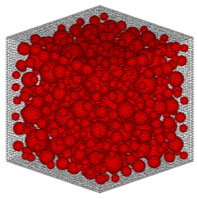
\includegraphics[width=.6\linewidth]{Files/exp_3D/A30Undamaged.png}
    \caption{Case 0: 0\% Expansion}
    \end{subfigure}%
    %*******
    \begin{subfigure}{.5\textwidth}
      \centering
      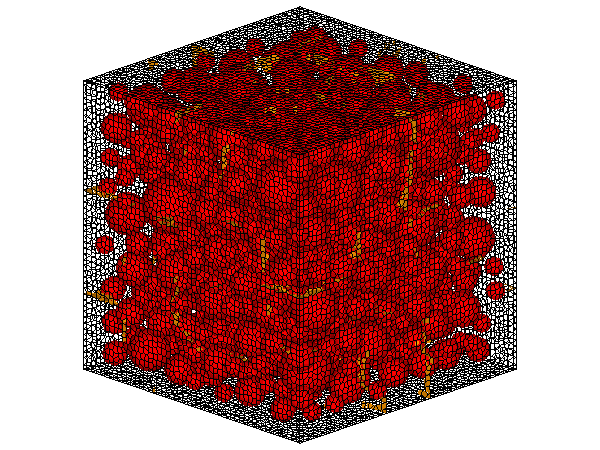
\includegraphics[width=.8\linewidth]{Files/exp_3D/DEF/A30X-5C_1_c.png}
    \caption{Case 1: 0.1671\% Expansion}
    \end{subfigure}
    %*******
    \begin{subfigure}{.5\textwidth}
      \centering
      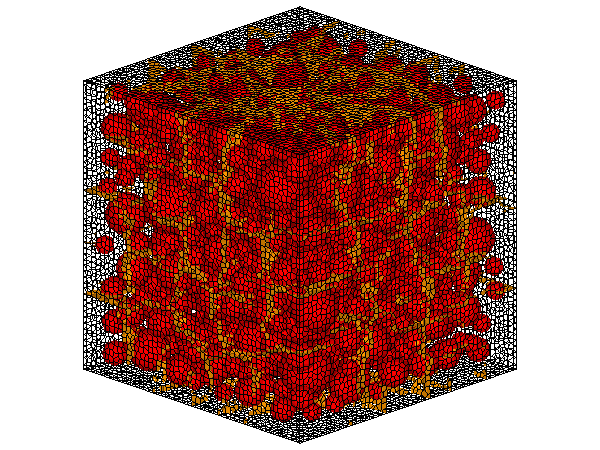
\includegraphics[width=.8\linewidth]{Files/exp_3D/DEF/A30X-5C_2_c.png}
    \caption{Case 2: 0.3380\% Expansion}
    \end{subfigure}%
    %*******
    \begin{subfigure}{.5\textwidth}
      \centering
      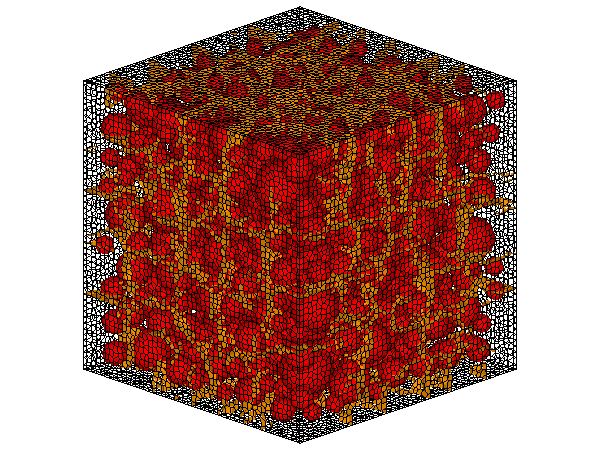
\includegraphics[width=.8\linewidth]{Files/exp_3D/DEF/A30X-5C_3_c.png}
    \caption{Case 3: 0.5118\% Expansion}
    \end{subfigure}
    %*******
    \begin{subfigure}{.5\textwidth}
      \centering
      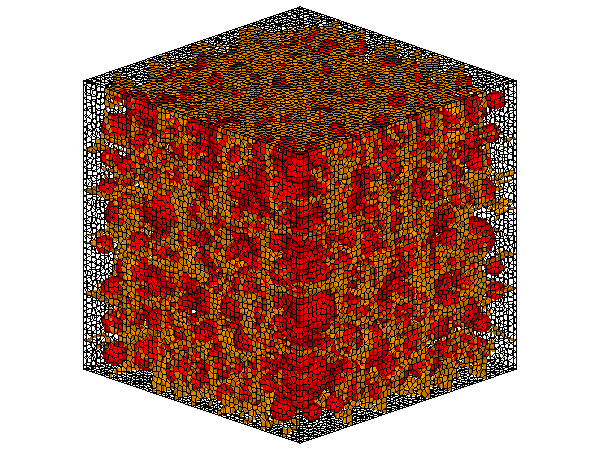
\includegraphics[width=.8\linewidth]{Files/exp_3D/DEF/A30X-5C_4_c.png}
    \caption{Case 4: 0.8577\% Expansion}
    \end{subfigure}%
    %*******

  \caption{3D Inner Cracks Expansion Intensified $75 \times 75 \times 75$ mm}
  \label{fig:DEF_A30X-5C_3Dasdasd}
\end{figure}


\clearpage
\subsubsection{Expansion Intensified $100 \times 100 \times 100$ mm at Center of Model}

Same trend of larger global expansion in $100 \times 100 \times 100$ mm case can also be seen in Tabel \ref{table:DEF_X-1_EssXP} and \ref{fig:DEFA30X0vsX-1_exssp}.

However, when comparing to uniformed overall expansion (DEF expansion at the center $75 \times 75 \times 75$ mm), as shown in Figure \ref{fig:DEF_A30X-1C_3Dss}, Figure \ref{fig:DEF_A30X-1C_3DssS} and Figure \ref{fig:DEF_A30X-1C_3Dcasd},the increasing of the concrete volume is achieved without generating significant surface cracks. This simulation result is correlated with the research result done by L.Eddy et.al., 2016\cite{Eddy}, concluded as the simply uniformed paste expansion does not present DEF simulation well as it behaves in reality.

\begin{table}[ht!]
  \caption{Global Expansion vs. Initial Strain Given in Each Step}
\centering
\begin{tabular}{ ||p{2cm}|p{2cm}|p{2cm}| }
 \hline
    Initial Strain (Each Step) & Expanding Steps &  Final Expansion[\%] \\ [0.5ex]
 \hline\hline
  0 & 0 & 0 \\
  0.001 & 20 & 0.2 \\
  0.002 & 20 & 0.4087 \\
  0.004 & 20 & 0.6191 \\
  0.006 & 20 & 1.0454 \\
 \hline
\end{tabular}

\label{table:DEF_X-1_EssXP}
\end{table}

\begin{figure}[ht!]
\centering
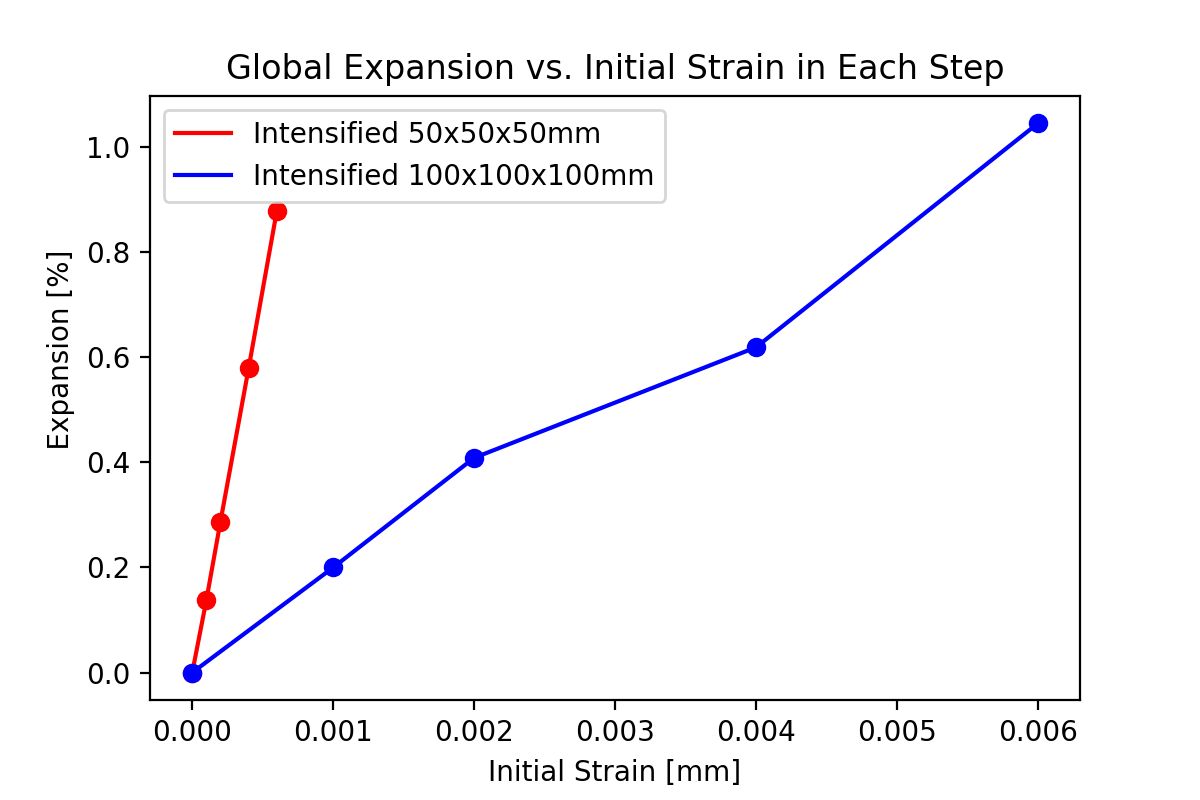
\includegraphics[width=.8\linewidth]{Files/exp_plot/DEFA30X0vsX-1_exp.png}
\caption{One Dimensional Expansion Ratio[\%] in Expansion Intensified $100 \times 100 \times 100$ mm at Center of Model DEF Model Simulation}
\label{fig:DEFA30X0vsX-1_exssp}
\end{figure}
\begin{figure}[ht!]
\centering

    %*******
    \begin{subfigure}{.5\textwidth}
      \centering
      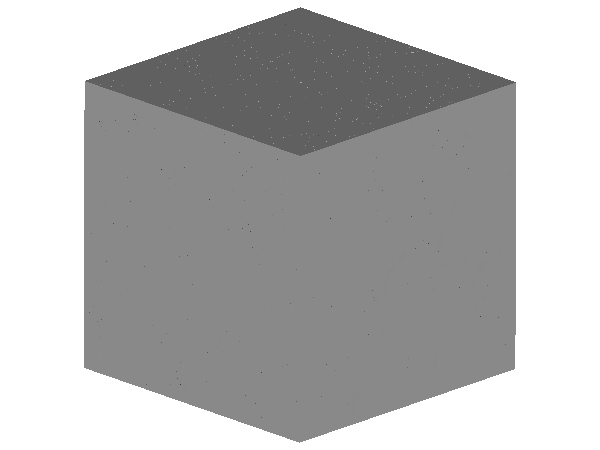
\includegraphics[width=.8\linewidth]{Files/exp_3D/ASR/A30Undamaged.png} %TODO: Fix. Should be A30
    \caption{Case 0: 0\% Expansion}
    \end{subfigure}%
    %*******
    \begin{subfigure}{.5\textwidth}
      \centering
      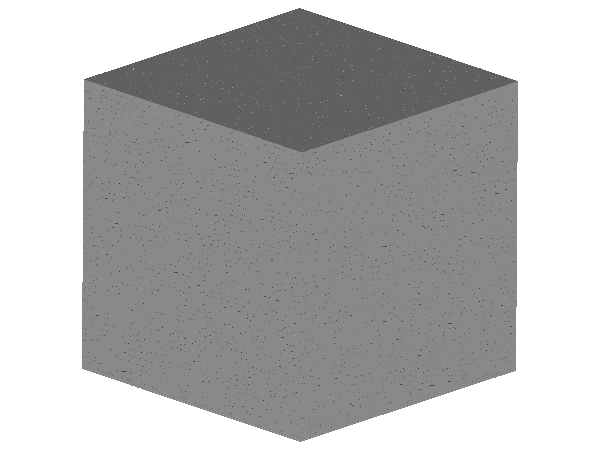
\includegraphics[width=.8\linewidth]{Files/exp_3D/DEF/A30X-1C_1_3d.png}
    \caption{Case 1: 0.2\% Expansion}
    \end{subfigure}
    %*******
    \begin{subfigure}{.5\textwidth}
      \centering
      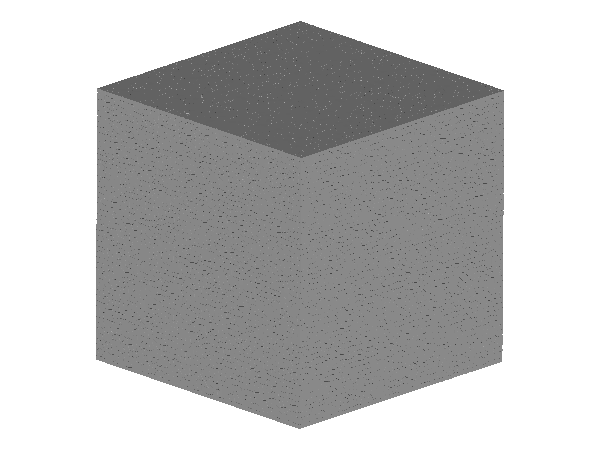
\includegraphics[width=.8\linewidth]{Files/exp_3D/DEF/A30X-1C_2_3d.png}
    \caption{Case 2: 0.4087\% Expansion}
    \end{subfigure}%
    %*******
    \begin{subfigure}{.5\textwidth}
      \centering
      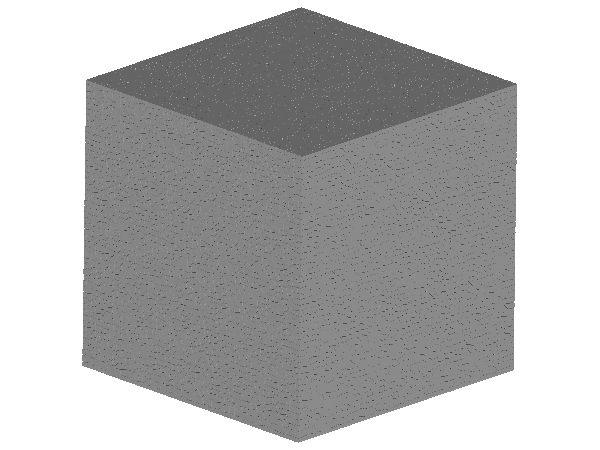
\includegraphics[width=.8\linewidth]{Files/exp_3D/DEF/A30X-1C_3_3d.png}
    \caption{Case 3: 0.6191\% Expansion}
    \end{subfigure}
    %*******
    \begin{subfigure}{.5\textwidth}
      \centering
      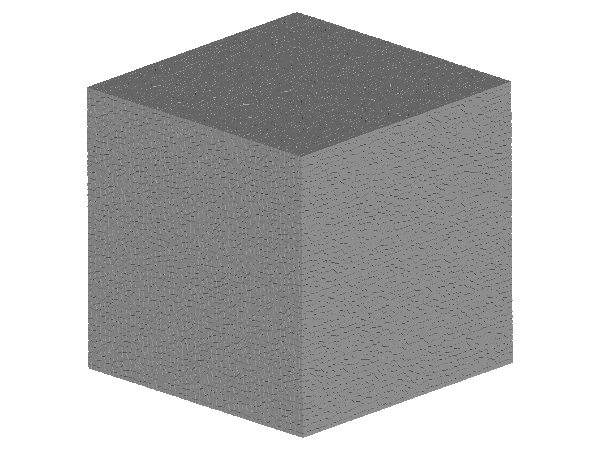
\includegraphics[width=.8\linewidth]{Files/exp_3D/DEF/A30X-1C_4_3d.png}
    \caption{Case 4: 1.0454\% Expansion}
    \end{subfigure}%
    %*******

  \caption{3D Surface Cracks Expansion Intensified $100 \times 100 \times 100$ mm ($Deformation \times 10$)}
  \label{fig:DEF_A30X-1C_3Dss}
\end{figure}

% Surface of one side
\begin{figure}[ht!]
\centering

    %*******
    \begin{subfigure}{.5\textwidth}
      \centering
      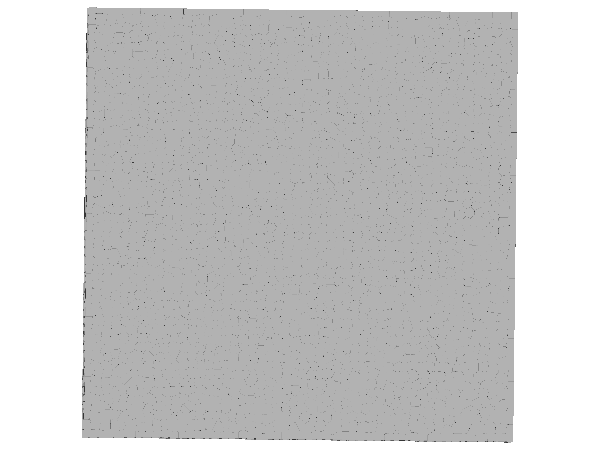
\includegraphics[width=.8\linewidth]{Files/exp_3D/DEF/A30X-1C_1_3ds.png}
    \caption{Case 0: 0\% Expansion}
    \end{subfigure}%
    %*******
    \begin{subfigure}{.5\textwidth}
      \centering
      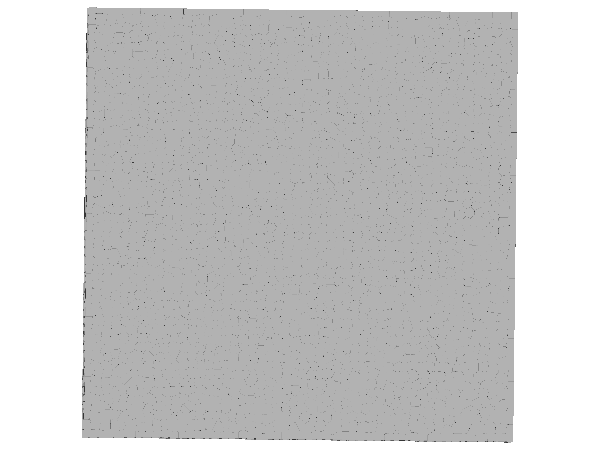
\includegraphics[width=.8\linewidth]{Files/exp_3D/DEF/A30X-1C_1_3ds.png}
    \caption{Case 1: 0.2\% Expansion}
    \end{subfigure}
    %*******
    \begin{subfigure}{.5\textwidth}
      \centering
      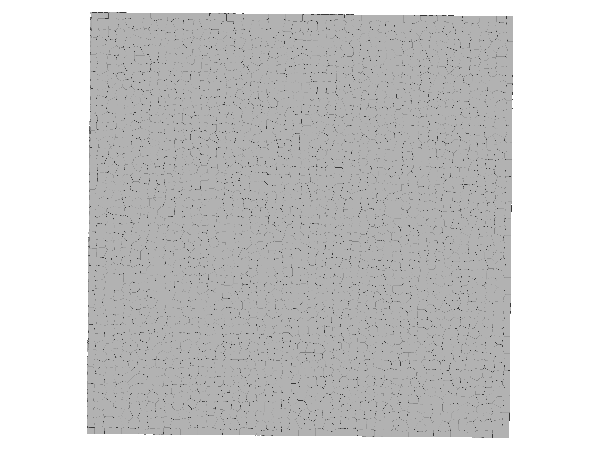
\includegraphics[width=.8\linewidth]{Files/exp_3D/DEF/A30X-1C_2_3ds.png}
    \caption{Case 2: 0.4087\% Expansion}
    \end{subfigure}%
    %*******
    \begin{subfigure}{.5\textwidth}
      \centering
      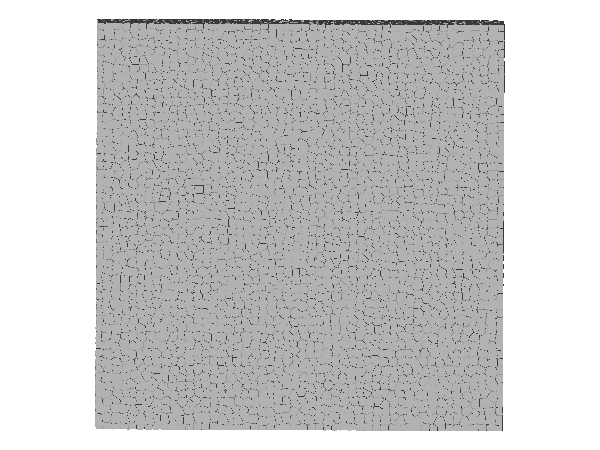
\includegraphics[width=.8\linewidth]{Files/exp_3D/DEF/A30X-1C_3_3ds.png}
    \caption{Case 3: 0.6191\% Expansion}
    \end{subfigure}
    %*******
    \begin{subfigure}{.5\textwidth}
      \centering
      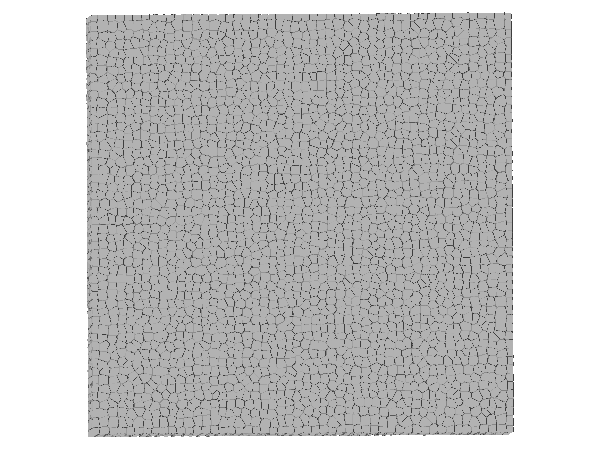
\includegraphics[width=.8\linewidth]{Files/exp_3D/DEF/A30X-1C_4_3ds.png}
    \caption{Case 4: 1.0454\% Expansion}
    \end{subfigure}%

  \caption{3D Surface Cracks (Single Side View) Expansion Intensified $100 \times 100 \times 100$ mm ($Deformation \times 10$)}
  \label{fig:DEF_A30X-1C_3DssS}
\end{figure}

\begin{figure}[ht!]
\centering

    %*******
    \begin{subfigure}{.5\textwidth}
      \centering
      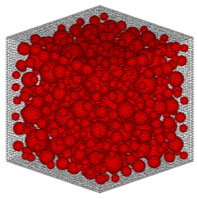
\includegraphics[width=.6\linewidth]{Files/exp_3D/A30Undamaged.png}
    \caption{Case 0: 0\% Expansion}
    \end{subfigure}%
    %*******
    \begin{subfigure}{.5\textwidth}
      \centering
      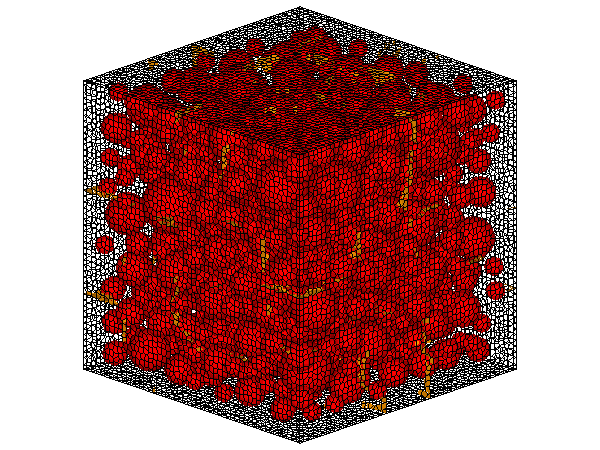
\includegraphics[width=.8\linewidth]{Files/exp_3D/DEF/A30X-1C_1_c.png}
    \caption{Case 1: 0.2\% Expansion}
    \end{subfigure}
    %*******
    \begin{subfigure}{.5\textwidth}
      \centering
      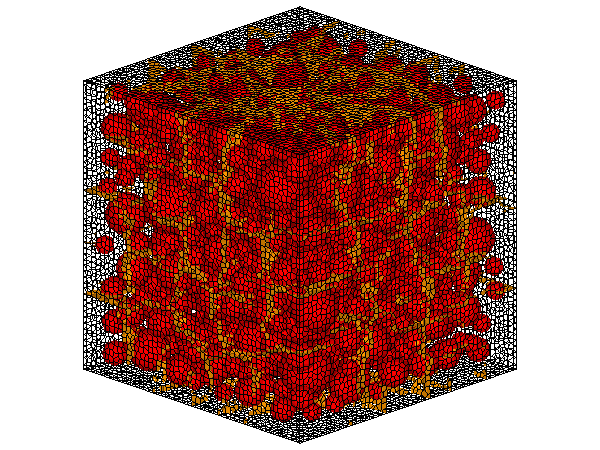
\includegraphics[width=.8\linewidth]{Files/exp_3D/DEF/A30X-1C_2_c.png}
    \caption{Case 2: 0.4087\% Expansion}
    \end{subfigure}%
    %*******
    \begin{subfigure}{.5\textwidth}
      \centering
      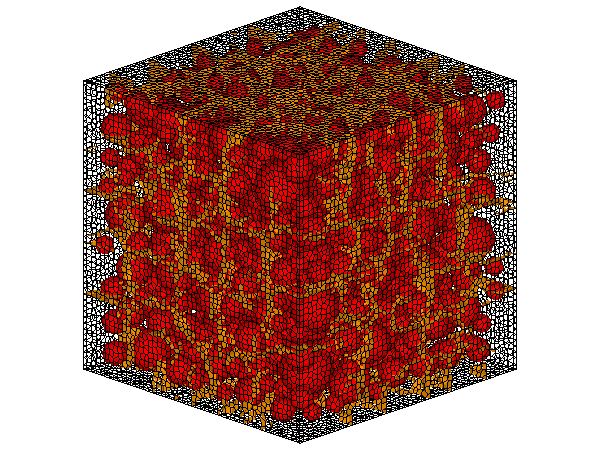
\includegraphics[width=.8\linewidth]{Files/exp_3D/DEF/A30X-1C_3_c.png}
    \caption{Case 3: 0.6191\% Expansion}
    \end{subfigure}
    %*******
    \begin{subfigure}{.5\textwidth}
      \centering
      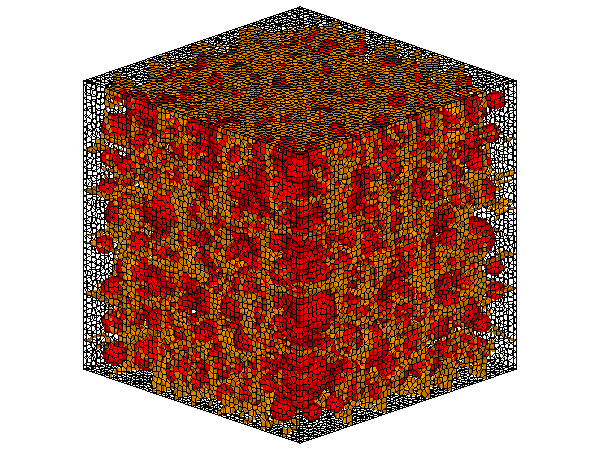
\includegraphics[width=.8\linewidth]{Files/exp_3D/DEF/A30X-1C_4_c.png}
    \caption{Case 4: 1.0454\% Expansion}
    \end{subfigure}%
    %*******

  \caption{3D Inner Cracks Expansion Intensified $100 \times 100 \times 100$ mm ($Deformation \times 10$)}
  \label{fig:DEF_A30X-1C_3Dcasd}
\end{figure}

\clearpage

\begin{figure}[ht!]
\centering
    %*******
    \begin{subfigure}{.3\textwidth}
      \centering
      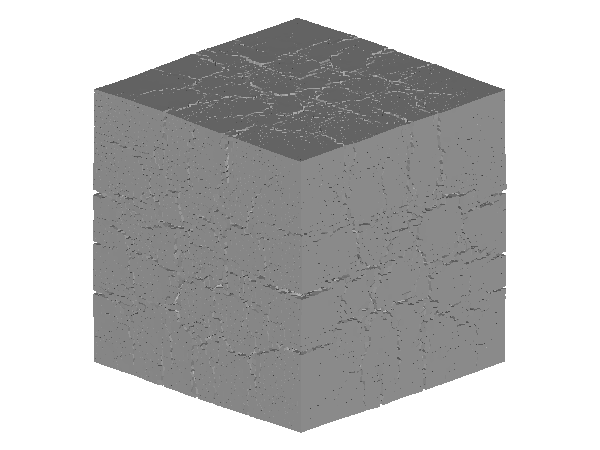
\includegraphics[width=.9\linewidth]{Files/exp_3D/DEF/A30X0C_3_3d.png}
    \caption{Intensified $50 \times 50 \times 50$ mm \\ 0.5795\% Expansion}
    \end{subfigure}%
    %*******
    \begin{subfigure}{.3\textwidth}
      \centering
      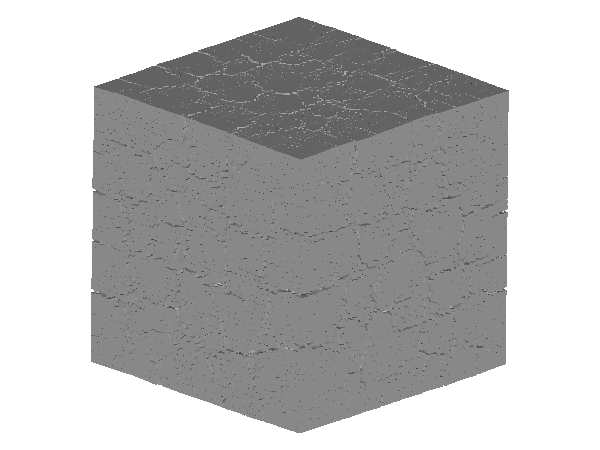
\includegraphics[width=.9\linewidth]{Files/exp_3D/DEF/A30X-5C_3_3d.png}
    \caption{Intensified $75 \times 75 \times 75$ mm \\  0.5118\% Expansion}
    \end{subfigure}
    %*******
    \begin{subfigure}{.3\textwidth}
      \centering
      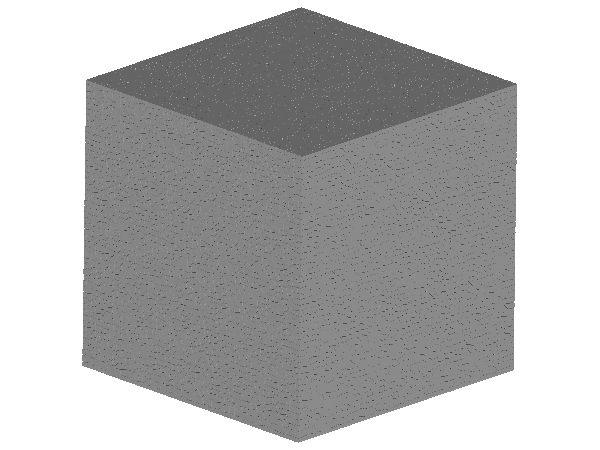
\includegraphics[width=.9\linewidth]{Files/exp_3D/DEF/A30X-1C_3_3d.png}
    \caption{Intensified $100 \times 100 \times 100$ mm \\  0.6191\% Expansion}
    \end{subfigure}%
    %*******

    %*******
    \begin{subfigure}{.3\textwidth}
      \centering
      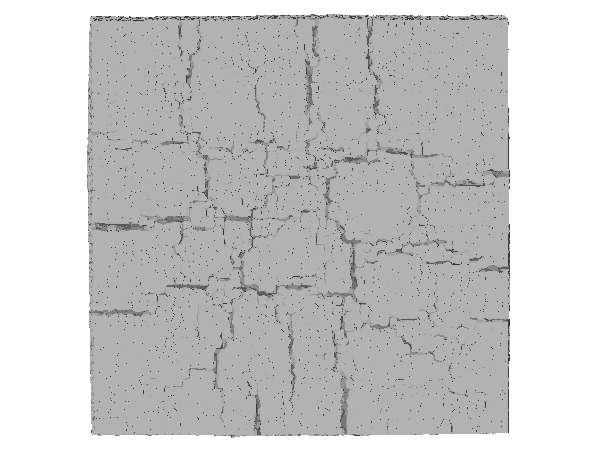
\includegraphics[width=.9\linewidth]{Files/exp_3D/DEF/A30X0C_3_3ds.png}
    \caption{Intensified $50 \times 50 \times 50$ mm \\  0.5795\% Expansion}
    \end{subfigure}%
    %*******
    \begin{subfigure}{.3\textwidth}
      \centering
      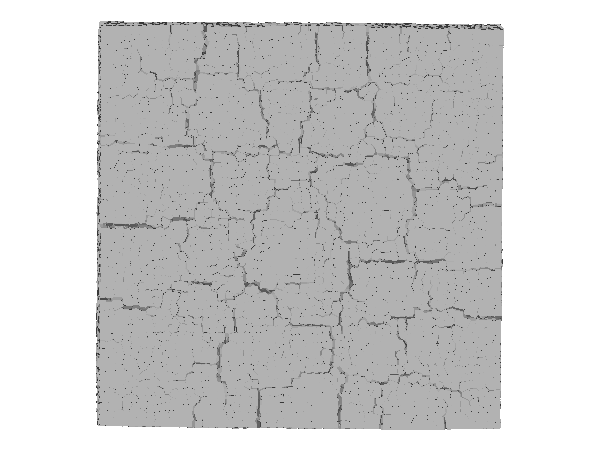
\includegraphics[width=.9\linewidth]{Files/exp_3D/DEF/A30X-5C_3_3ds.png}
    \caption{Intensified $75 \times 75 \times 75$ mm \\  0.5118\% Expansion}
    \end{subfigure}
    %*******
    \begin{subfigure}{.3\textwidth}
      \centering
      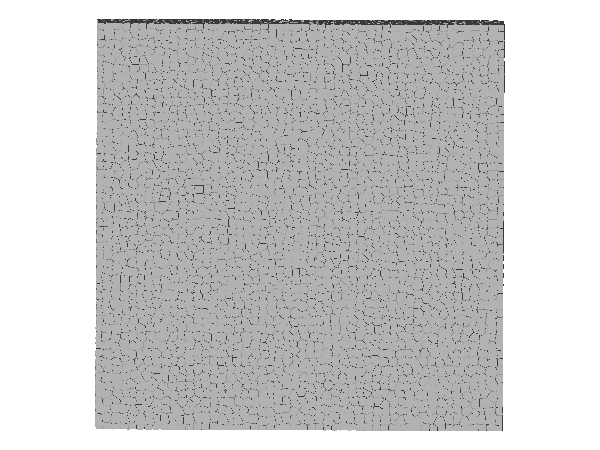
\includegraphics[width=.9\linewidth]{Files/exp_3D/DEF/A30X-1C_3_3ds.png}
    \caption{Intensified $100 \times 100 \times 100$ mm  \\ 0.6191\% Expansion}
    \end{subfigure}%
    %*******

    %*******
    \begin{subfigure}{.3\textwidth}
      \centering
      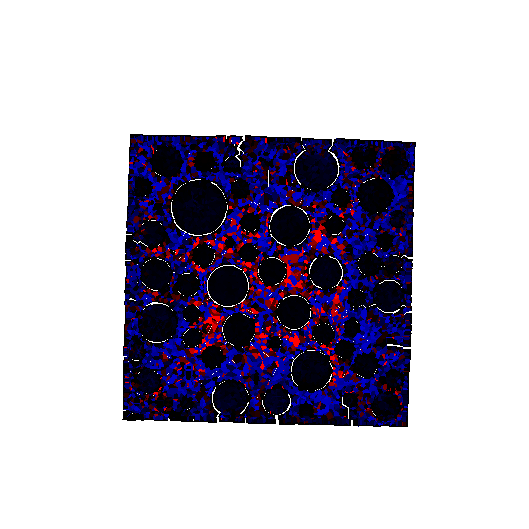
\includegraphics[width=.9\linewidth]{Files/exp_3D/DEF/A30X0C_3_stress.png}
    \caption{Intensified $50 \times 50 \times 50$ mm \\  0.5795\% Expansion}
    \end{subfigure}%
    %*******
    \begin{subfigure}{.3\textwidth}
      \centering
      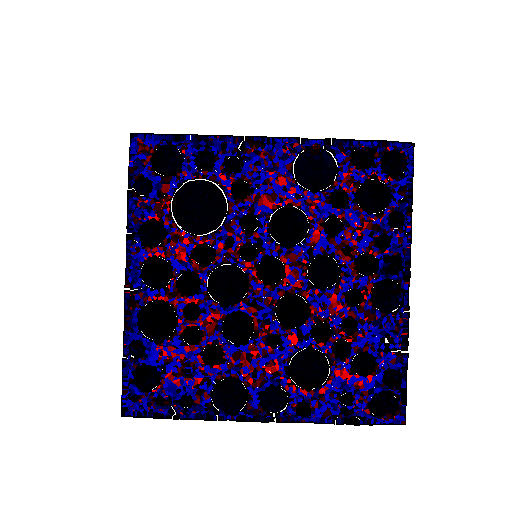
\includegraphics[width=.9\linewidth]{Files/exp_3D/DEF/A30X-5C_3_stress.png}
    \caption{Intensified $75 \times 75 \times 75$ mm  \\ 0.5118\% Expansion}
    \end{subfigure}
    %*******
    \begin{subfigure}{.3\textwidth}
      \centering
      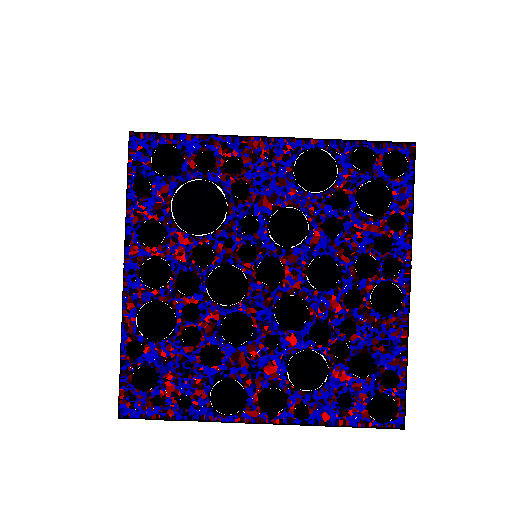
\includegraphics[width=.9\linewidth]{Files/exp_3D/DEF/A30X-1C_3_stress.png}
    \caption{Intensified $100 \times 100 \times 100$ mm \\  0.6191\% Expansion}
    \end{subfigure}%
    %*******

    %*******
    \begin{subfigure}{.3\textwidth}
      \centering
      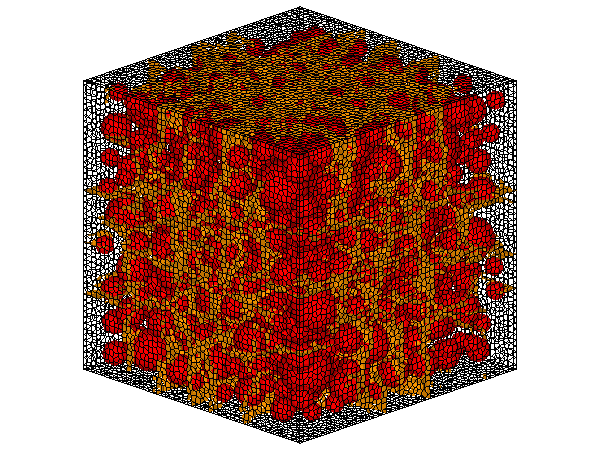
\includegraphics[width=.9\linewidth]{Files/exp_3D/DEF/A30X0C_3_c.png}
    \caption{Intensified $50 \times 50 \times 50$ mm \\  0.5795\% Expansion}
    \end{subfigure}%
    %*******
    \begin{subfigure}{.3\textwidth}
      \centering
      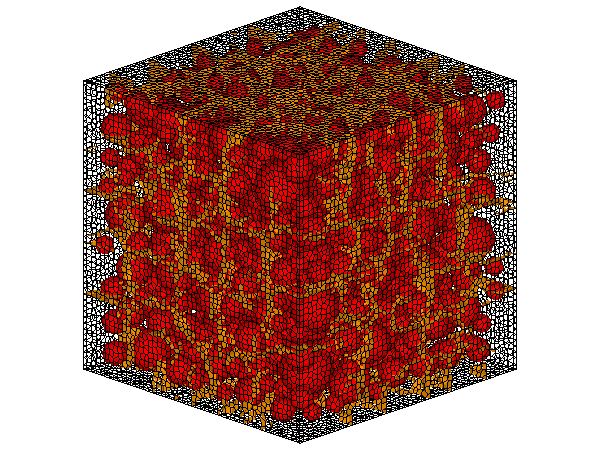
\includegraphics[width=.9\linewidth]{Files/exp_3D/DEF/A30X-5C_3_c.png}
    \caption{Intensified $75 \times 75 \times 75$ mm  \\ 0.5118\% Expansion}
    \end{subfigure}
    %*******
    \begin{subfigure}{.3\textwidth}
      \centering
      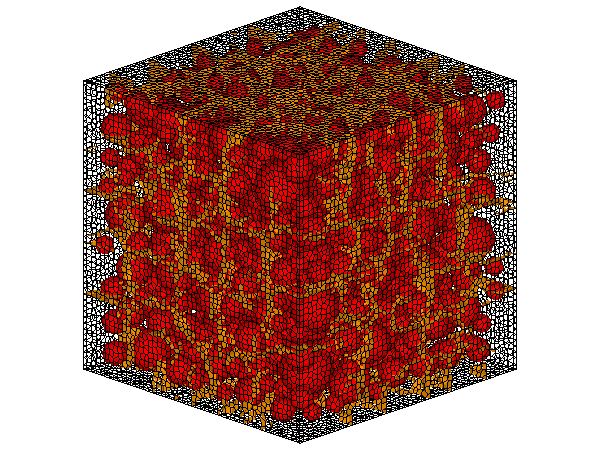
\includegraphics[width=.9\linewidth]{Files/exp_3D/DEF/A30X-1C_3_c.png}
    \caption{Intensified $100 \times 100 \times 100$ mm \\  0.6191\% Expansion}
    \end{subfigure}%
    %*******

  \caption{Comparing between different DEF Expansion Intensified Cases}
  \label{fisg:DEF_X_compare}
\end{figure}


As shown in Figure \ref{fisg:DEF_X_compare}, when examined closely of the intersection, it can be seen that no inner crack is happening in the paste for the uniformed expanding case, separation only happens between the surface of aggregate and paste, which is different with other 2 cases.

With expansion intensified in the inner part of concrete model, the compressive force concentrated in the inner part of the model, while outer parts are under tension. This unbalanced force generates cracks at the surrounding part of the concrete, preset as map cracking pattern at the surface view. This cracking pattern is also correlated with the observation form A.Awasthi in his investigation of DEF deteriorated in Indian concrete sleeper in 2016\cite{Awasthi}.
